\documentclass[12pt, a4paper, oneside]{ctexart}
\usepackage{amsmath, amsthm, amssymb, bm, color, graphicx, geometry, hyperref, mathrsfs,extarrows, braket, booktabs, array}
\setmainfont{Times New Roman}  % 设置英文字体
\setsansfont{Calibri}
\setmonofont{Consolas}

\linespread{1.4}
%\geometry{left=2.54cm,right=2.54cm,top=3.18cm,bottom=3.18cm}
\geometry{left=1.84cm,right=1.84cm,top=2.18cm,bottom=2.18cm}
\newenvironment{problem}{\par\noindent\textbf{题目. }}{\bigskip\par}
\newenvironment{solution}{\par\noindent\textbf{解答. }}{\bigskip\par}
\newenvironment{note}{\par\noindent\textbf{注记. }}{\bigskip\par}

\everymath{\displaystyle} % 默认全部行间公式
\DeclareMathOperator*\uplim{\overline{lim}} % 定义上极限 \uplim_{}
\DeclareMathOperator*\lowlim{\underline{lim}} % 定义下极限 \lowlim_{}
\let\leq=\leqslant % 将全部leq变为leqslant
\let\geq=\geqslant % geq同理

% 一些宏定义
\def\bd{\boldsymbol}    % 加粗(向量) boldsymbol
\def\disp{\displaystyle}% 使用行间公式 displaystyle(默认)
\def\tsty{\textstyle}   % 使用行内公式 textstyle
\def\sign{\text{sign}}  % sign function
\def\wtd{\widetilde}    % 宽波浪线 widetilde
\def\R{\mathbb{R}}      % Real number
\def\C{\mathbb{C}}      % Complex number
\def\d{\mathrm{d}}      % differential operator
\def\e{\mathrm{e}}      % Euler's number
\def\i{\mathrm{i}}      % imaginary number
\def\L{\mathcal{L}}     % Loss function
\def\wdh{\widehat}      % 宽帽子 widehat
\def\ol{\overline}      % 上横线 overline
\def\ul{\underline}     % 下横线 underline
\def\add{\vspace{0.5ex}}  % 增加行间距
\def\del{\vspace{-3.5ex}}  % 减少行间距

% 基本信息
\newcommand{\RQ}{\today} % 日期
\newcommand{\km}{实变函数} % 科目
\newcommand{\bj}{强基数学002} % 班级
\newcommand{\xm}{吴天阳} % 姓名
\newcommand{\xh}{2204210460} % 学号
\newcommand{\XH}{59} % 序号

\begin{document}

%\pagestyle{empty}
\pagestyle{plain}
\vspace*{-15ex}
\centerline{\begin{tabular}{*6{c}}
    \parbox[t]{0.25\linewidth}{\begin{center}\textbf{日期}\\ \large \textcolor{blue}{\RQ}\end{center}} 
    & \parbox[t]{0.15\linewidth}{\begin{center}\textbf{科目}\\ \large \textcolor{blue}{\km}\end{center}}
    & \parbox[t]{0.2\linewidth}{\begin{center}\textbf{班级}\\ \large \textcolor{blue}{\bj}\end{center}}
    & \parbox[t]{0.1\linewidth}{\begin{center}\textbf{姓名}\\ \large \textcolor{blue}{\xm}\end{center}}
    & \parbox[t]{0.15\linewidth}{\begin{center}\textbf{学号}\\ \large \textcolor{blue}{\xh}\end{center}}
    & \parbox[t]{0.1\linewidth}{\begin{center}\textbf{序号}\\ \large \textcolor{blue}{\XH}\end{center}} \\ \hline
\end{tabular}}
\vspace*{4ex}

% 正文部分
\paragraph{习题3.1}
\paragraph{2.}设$(X,\bd{R})$是可测空间, $E_1,\cdots, E_n$是有限个可测集. 证明: $f$在$E=\bigcup_{i=1}^nE_i$上是可测的充要条件是$f$在每个$E_i(i=1,2,\cdots, n)$上是可测的. 再证上述命题对于$\{E_i\}$是一列可测集也是正确的.
\begin{proof}
    令$G_i = E_i-\bigcup_{j=1}^{i-1}E_j$, 则$E_i = \bigcup_{j=1}^iG_j$. 所以$f$在$E$上可测$\iff$$f$在$G_i(i=1,2,\cdots, n)$上可测$\iff$$f$在$E_i$上可测, 类似可证明$\{E_i\}$是一列可测集也是正确的.
\end{proof}
\paragraph{3.}设$X,\bd{R}$是可测空间, $E\subset X$. 证明$f$是$E$上可测函数的充要条件是对一切有理数$r$, $E(f\geq r)$是可测集.
\begin{proof}
    $f$为$E$上的可测函数$\iff$对于任意的$c\in\R$, $E(f\geq c)$为可测集$\iff$$E(f\geq c) = \bigcup_{n=1}^\infty E\left(f\geq \frac{[nc]}{n}\right)\in \bd{R}$.
\end{proof}
\paragraph{4.}设$(X,\bd{R})$是可测空间, $E\subset X$, $f$是$E$上有界可测函数. 证明必存在可测集的特征函数线性组合形式的函数序列$\{f_n\}$在$E$上一致收敛于$f$, 并且$|f_n(x)|\leq \sup_{x\in E}|f(x)|(n=1,2,3,\cdots)$.
\begin{proof}
    类似\textbf{定理}$3.1.6$证明: 构造$f_n = \sum_{j=-n^2}^{n^2-1}\frac{j}{n}\chi_{E_j^{(n)}}$, 其中$E_j^{(n)} = E\left(\frac{j}{n}\leq f < \frac{j+1}{n}\right)$. 令$M=\sup_{x\in E}|f(x)|$, 则当$n > M$时, $\forall x\in E$, 总有$j(x)\in [-n^2, n^2-1]$使得
    \begin{equation*}
        f_n(x)=\frac{j(x)}{n}\leq f(x) < \frac{j(x)+1}{n},
    \end{equation*}
    于是$f_n(x)\leq \sup_{x\in E}|f(x)|$, 即$x\in E_{j(x)}^{(n)}$, 由$f_n$构造法知, $f_n(x) = \frac{j(x)}{n}$, 则当$n\to \infty$时, 有
    \begin{equation*}
        |f(x)-f_n(x)| < \left| f(x)-\frac{j(x)}{n}\right|<\frac{1}{n}\to 0\qquad(\forall x \in E).
    \end{equation*}
\end{proof}
\paragraph{6.}设$(X,\bd{R})$是可测空间, $E\subset X)$, $f$是$E$上可测函数. 又设$h$是直线上Borel可测函数, 证明$h(f)$是$E$上可测函数.
\begin{proof}
    设$a<b$, 则
    \begin{equation*}
        f^{-1}((a,b)) = \{x\in E:a<f(x)<b\} = \{x\in E:f(x) > a\}\cap\{x\in E:f(x) < b\}\in \bd{R}.
    \end{equation*}
    设$\{(a_i,b_i)\}$为一列开集族, $G = \bigcup_{i=1}^\infty(a_i,b_i)$, 则
    \begin{equation*}
        f^{-1}(G) = f^{-1}\left(\bigcup_{i=1}^\infty(a_i, b_i)\right) = \bigcup_{i=1}^\infty f^{-1}(a_i,b_i)\in \bd{R},
    \end{equation*}
    设$F = E^1 - G$, 则
    \begin{equation*}
        f^{-1}(F) = f^{-1}(E^1-G) = E-f^{-1}(G) \in \bd{R}.
    \end{equation*}
    设$\mathcal{A} = \{A\subset E^1:f^{-1}(A)\text{可测}\}$, 则当$A_n\in\mathcal{A}$, $n=1,2,\cdots$时
    \begin{align*}
        &\ f^{-1}(A_1-A_2)= f^{-1}(A_1)-f^{-1}(A_2)\in \bd{R},\\
        &\ f^{-1}\left(\bigcup_{i=1}^\infty A_i\right) = \bigcup_{i=1}^\infty f^{-1}(A_i)\in \bd{R},\\
        &\ f^{-1}(E^1) = E\in \bd{R}.
    \end{align*}
    由于Borel集$\mathcal{B}\subset\mathcal{A}$, 于是任何Borel集$M$, $f^{-1}(M)\in\bd{R}$.
    $h$为Borel可测函数, 
    \begin{equation*}
        h^{-1}([c,\infty)) = \{x\in \R:h(x)\geq c\}\in \mathcal{B},
    \end{equation*}
    所以
    \begin{equation*}
        E(h\circ f\geq c) = \{x\in E: h(f(x))\geq c\} = (h\circ f)^{-1}([c,\infty)) = f^{-1}(h^{-1}([c, \infty)))\in \bd{R}.
    \end{equation*}
\end{proof}
\paragraph{7.}设$(X,\bd{R})$是可测函数, $E\subset X,\{f_n\}$是$E$上一列有限的可测函数, 并且$\{f_n\}$在$E$上处处收敛(允许极限值是$\pm\infty$)$f$. 证明$E(f=\infty),E(f=-\infty)$是可测集, 并且对任何实数$c$, $E(f\geq c)$也是可测集.
\begin{proof}
    由于$\lim_{n\to\infty}f_n = f$, 任意$k\in \mathbb{N},\exists N$使$\forall n\geq N$, 有$f_n > c-\frac{1}{k}$,
    \begin{align*}
        &E(f\geq c) = E\left(\lim_{n\to\infty}f_n\geq c\right) = \bigcap_{k=1}^\infty\bigcup_{N=1}^\infty\bigcap_{n=N}^\infty E(f_n\geq c)\in \bd{R},\\
        &E(f=\infty) = \bigcap_{m=1}^\infty E(f\geq m)\in \bd{R},\\
        &E(f = -\infty) = E(-f=\infty)\in\bd{R}.
    \end{align*}
\end{proof}

% 下面给一些功能的写法
\iffalse
% 图片模板
\centerline{
    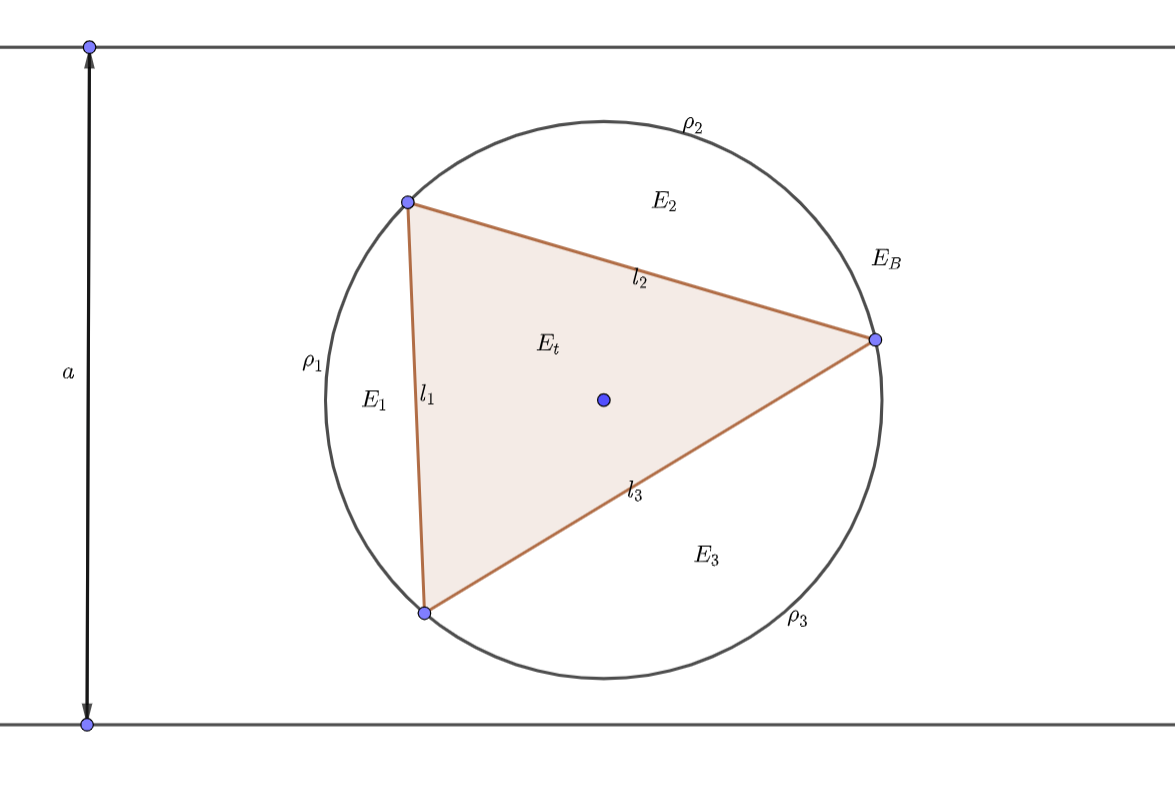
\includegraphics[width=0.8\textwidth]{figure.png}
}
% 表格模板
\renewcommand\arraystretch{0.8} % 设置表格高度为原来的0.8倍
\begin{table}[!htbp] % table标准
    \centering % 表格居中
    \begin{tabular}{p{1cm}<{\centering}p{1cm}<{\centering}p{3cm}<{\centering}p{5cm}<{\centering}} % 设置表格宽度
    %\begin{tabular}{cccc}
        \toprule
        $x_i$ & $f[x_1]$ & $f[x_i,x_{i+1}]$ & $f[x_i,x_{i+1},x_{i+2}]$ \\
        \midrule
        $x_0$ & $f(x_0)$ &                  &                          \\
        $x_0$ & $f(x_0)$ & $f'(x_0)$        &                          \\
        $x_0$ & $f(x_1)$ & $\frac{f(x_1)-f(x_0)}{x_1-x_0}$ & $\frac{f(x_1)-f(x_0)}{(x_1-x_0)^2}-\frac{f'(x_0)}{x_1-x_0}$\\
        \bottomrule
    \end{tabular}
\end{table}

\def\Log{\text{Log}} % 一个简单的宏定义
$\Log$ % 调用方法
\fi

\end{document}